%% The following is a directive for TeXShop to indicate the main file
%%!TEX root = diss.tex

\chapter{Motivation}
\label{ch:Motivation}
\begin{figure}
    \begin{subfigure}[t]{\textwidth}
        \makebox[\textwidth][c]{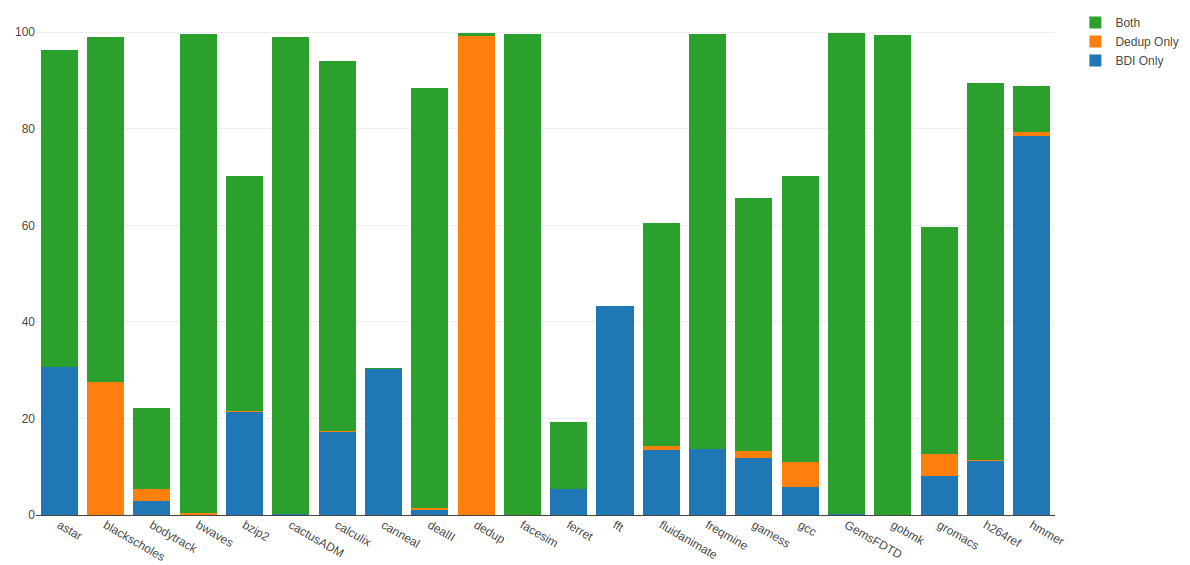
\includegraphics[width=1.5\textwidth]{CompPotential1.png}}
    \end{subfigure}
    \begin{subfigure}[b]{\textwidth}
        \makebox[\textwidth][c]{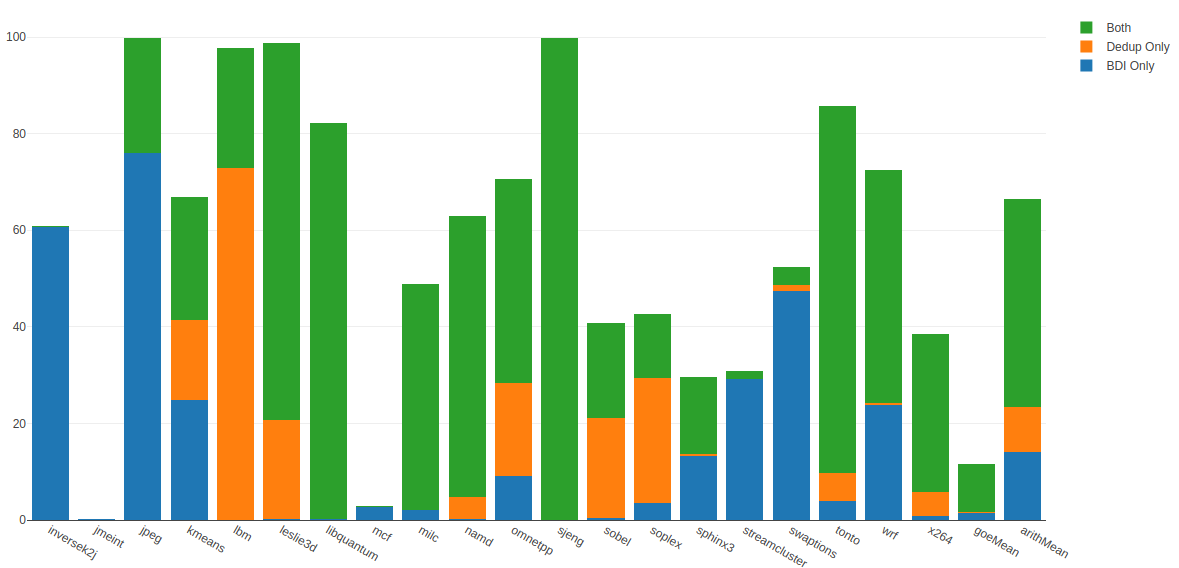
\includegraphics[width=1.5\textwidth]{CompPotential2.png}}
    \end{subfigure}
    \caption[Compressible lines]{The figure shows the percentage of cache lines that can be compressed using Dedup, BDI, or both techniques combined together.}
    \label{fig:CompPossibility}
\end{figure}
Deduplication and base delta immediate compression work on two different domains, one is inter-line and works on a cache line granularity while the other works intra-line with a granularity of two, four, or eight bytes. This means that they can both be combined to deduplicate similar lines and compress each of those lines at the same time. Figure \ref{fig:CompPossibility} shows the percentage of cache lines that can be compressed by BDI, the percentage of cache lines that are similar and thus deduplicable, and the percentage of cache lines that can be compressed using both schemes.\par
As Figure \ref{fig:CompPossibility} BDI and Deduplications are orthogonal to some degree. The existence of some cache lines that can be compressed by only one of both compression schemes means they can work separately without affecting each other. However, because there are lines that can be compressed by both schemes, BDI can lose some of it's improvements because of deduplication. For example, if ten lines were similar and compressible by BDI, using BDI will compress each of them on it's own, using deduplication will reduce all ten lines to only one line. Using both techniques means deduplication still compresses ten lines to one, but BDI now compresses only one line instead of 10. The improvements of BDI can thus be limited by deduplication.\par
\begin{figure}
    \begin{subfigure}[t]{\textwidth}
        \makebox[\textwidth][c]{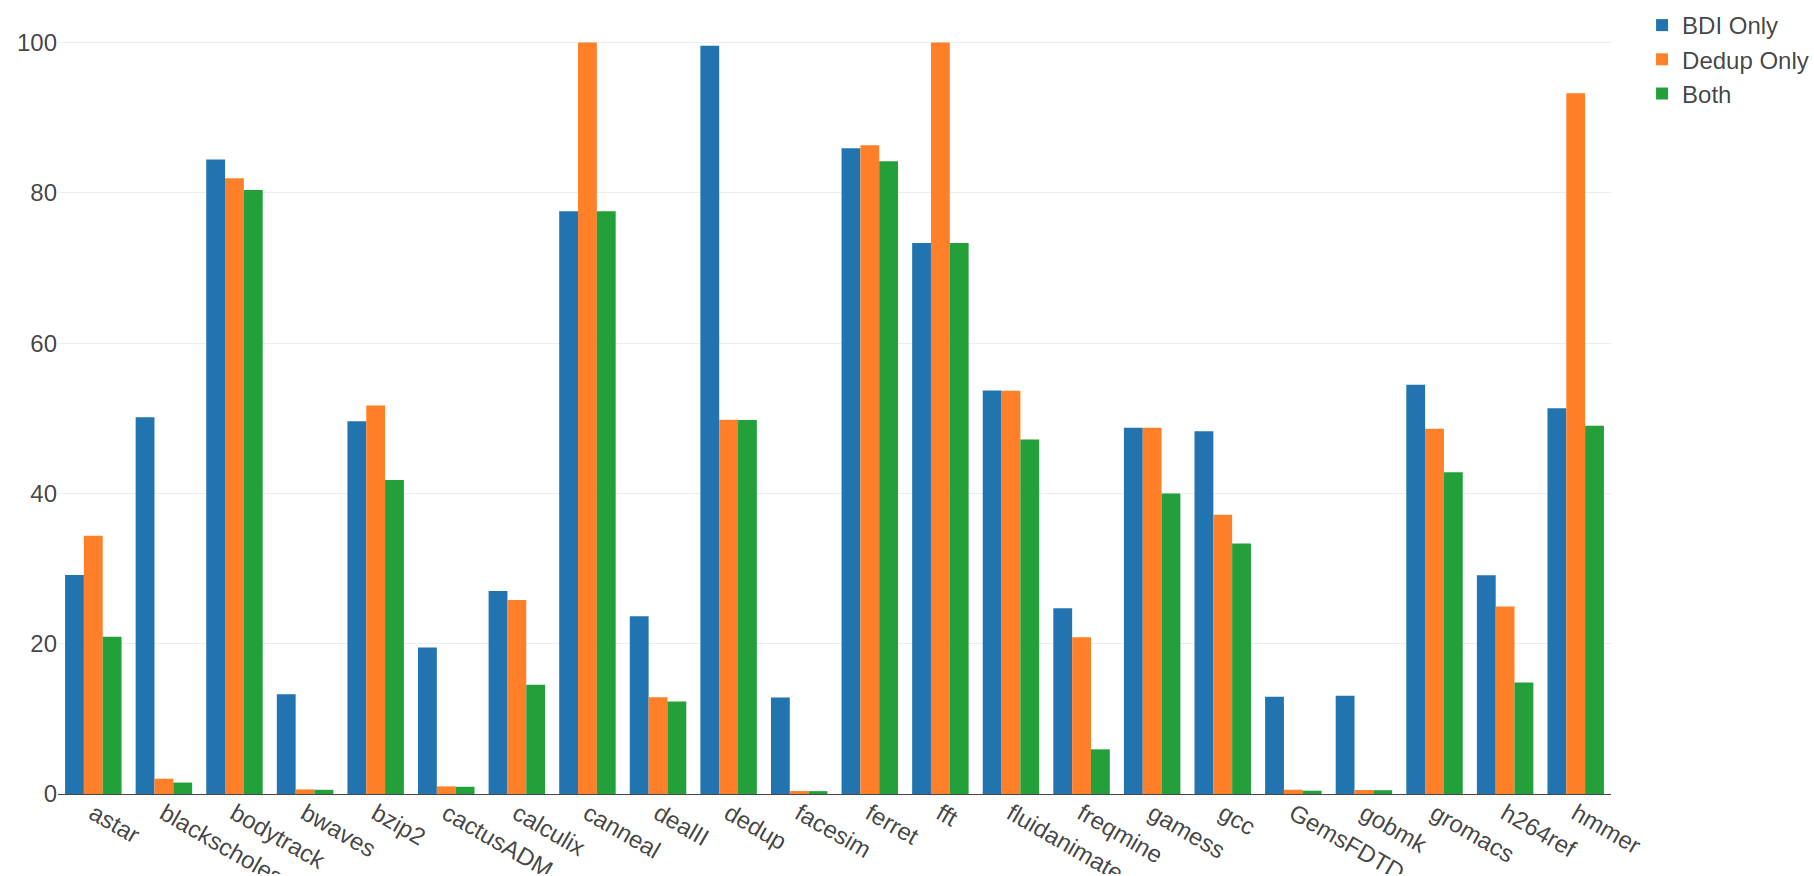
\includegraphics[width=1.5\textwidth]{CompSize1.png}}
    \end{subfigure}
    \begin{subfigure}[b]{\textwidth}
        \makebox[\textwidth][c]{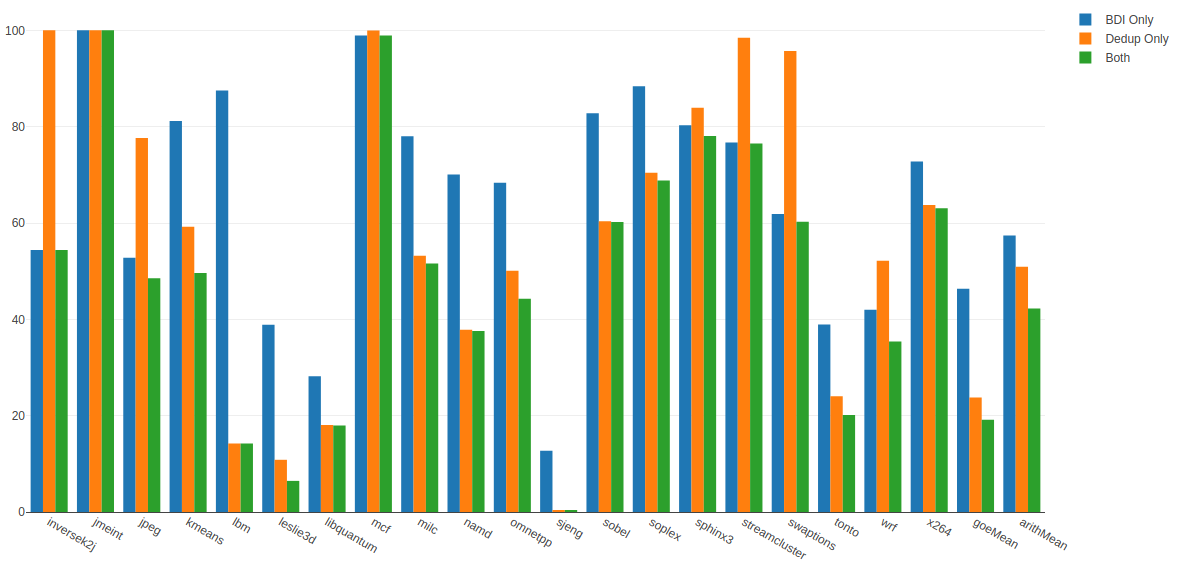
\includegraphics[width=1.5\textwidth]{CompSize2.png}}
    \end{subfigure}
    \caption[Size after compression]{The figure shows the size of data in a cache after using compression. BDI, Dedup, and a combination of both is shown.}
    \label{fig:CompSize}
\end{figure}
Nevertheless, combining BDI and Deduplication can still outperform each of them on its own. Figure \ref{fig:CompSize} shows the compressed data size when using BDI, Dedup, and Dedup+BDI. In its worst case Dedup+BDI performs the same as the best out of Dedup and BDI, in most cases it compresses even more on both. Note that the experiments used to create Figure \ref{fig:CompSize} are done statically on cache dumps and thus are completely missing the time dimension and its effect on compression. As time passes more requests to data lines can occur, with more requests the probability that compression can occur increases allowing for better compression.
